\documentclass{standalone}
\usepackage{tikz}
\usetikzlibrary{decorations.pathreplacing, arrows.meta}

\begin{document}

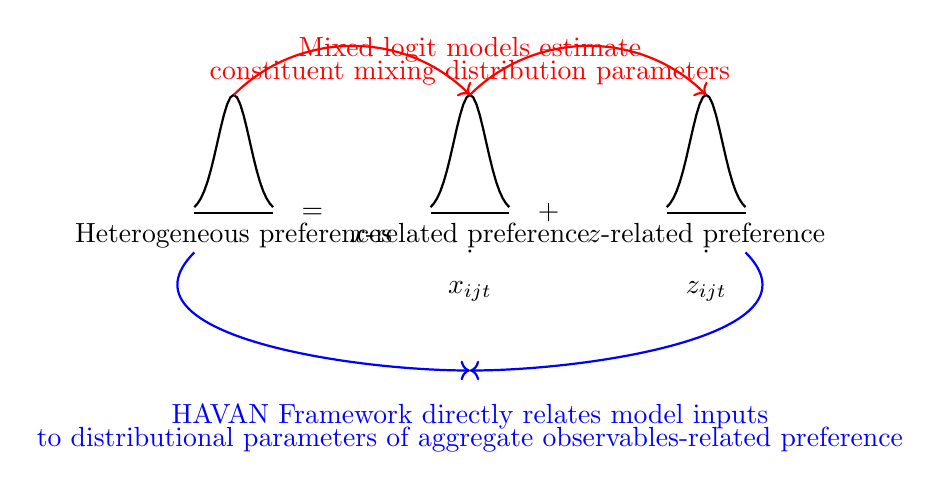
\begin{tikzpicture}

% Draw the normal distribution curves
\draw[thick] (0,0) -- (1,0) node[midway,below] {Heterogeneous preferences};
\draw[thick] plot[domain=0:1] (\x,{1.5*exp(-12*(\x-0.5)^2)});

\draw[thick] (3,0) -- (4,0) node[midway,below] {$x$-related preference};
\draw[thick] plot[domain=3:4] (\x,{1.5*exp(-12*(\x-3.5)^2)});

\draw[thick] (6,0) -- (7,0) node[midway,below] {$z$-related preference};
\draw[thick] plot[domain=6:7] (\x,{1.5*exp(-12*(\x-6.5)^2)});

% Add the mathematical symbols and variables
\node at (1.5,0) {$=$};
\node at (4.5,0) {$+$};
\node at (3.5,-0.5) {$\cdot$};
\node at (6.5,-0.5) {$\cdot$};
\node at (3.5,-1) {$x_{ijt}$};
\node at (6.5,-1) {$z_{ijt}$};

% Add the arrows and text
\draw[->, thick, red] (0.5,1.5) to[out=45,in=135] (3.5,1.5);
\draw[->, thick, red] (3.5,1.5) to[out=45,in=135] (6.5,1.5);
\node[red, above] at (3.5,1.8) {Mixed logit models estimate};
\node[red, above] at (3.5,1.5) {constituent mixing distribution parameters};

\draw[->, thick, blue] (0,-0.5) to[out=-135,in=180] (3.5,-2);
\draw[->, thick, blue] (7,-0.5) to[out=-45,in=0] (3.5,-2);
\node[blue, below] at (3.5,-2.3) {HAVAN Framework directly relates model inputs};
\node[blue, below] at (3.5,-2.6) {to distributional parameters of aggregate observables-related preference};

\end{tikzpicture}

\end{document}